\begingroup

% Hình UI chưa có tệp tương ứng sẽ hiện tên tệp cần bổ sung.
\newcommand{\insertfigure}[4]{%
  \begin{figure}[htbp]
  \centering
  \IfFileExists{#2}{\includegraphics[width=#1\linewidth]{s2/#2}}{\fbox{\texttt{#2}}}
  \caption{#3}
  \label{#4}
  \end{figure}%
}
\newcommand{\insertdiagram}[3]{%
  \begin{figure}[!htbp]
  \centering
  \includegraphics[width=0.96\linewidth,height=0.84\textheight,keepaspectratio]{s2/#1}
  \caption{#2}
  \label{#3}
  \end{figure}%
}
\newcommand{\insertsplitdiagram}[4]{%
  \begin{figure}[!htbp]
  \centering
  \includegraphics[width=0.48\linewidth,height=0.72\textheight,keepaspectratio]{s2/#1}\hfill
  \includegraphics[width=0.48\linewidth,height=0.72\textheight,keepaspectratio]{s2/#2}
  \caption{#3}
  \label{#4}
  \end{figure}%
}
\newcommand{\insertpair}[4]{%
  \begin{figure}[htbp]
  \centering
  \includegraphics[width=0.48\linewidth,height=0.72\textheight,keepaspectratio]{s2/#1}\hfill
  \includegraphics[width=0.48\linewidth,height=0.72\textheight,keepaspectratio]{s2/#2}
  \caption{#3}
  \label{#4}
  \end{figure}%
}
\newcommand{\insertmobilepair}[6]{%
  \begin{figure}[p]
  \centering
  \includegraphics[width=0.9\linewidth,height=0.4\textheight,keepaspectratio]{s2/#1}
  \captionof{figure}{#2}
  \label{#3}
  \par\vspace{0.4em}
  \includegraphics[width=0.9\linewidth,height=0.4\textheight,keepaspectratio]{s2/#4}
  \captionof{figure}{#5}
  \label{#6}
  \end{figure}%
}
\newcommand{\insertdashboardpair}[4]{%
  \begin{figure}[!htbp]
  \centering
  \includegraphics[width=0.99\linewidth,height=0.4\textheight,keepaspectratio]{s2/#1}
  \par\vspace{0.5em}
  \includegraphics[width=0.99\linewidth,height=0.4\textheight,keepaspectratio]{s2/#2}
  \caption{#3}
  \label{#4}
  \end{figure}%
}

\section{UI MOCKUP}

\subsection{Phân hệ Mobile App (Dành cho Sinh viên)}

\insertpair{UI/MapSearch.png}{UI/MapSearch_Dark.png}{Màn hình bản đồ và tìm kiếm Hub, phương tiện, trạm sạc ở giao diện sáng và tối (UC1, UC2).}{fig:map_search_screen}

\insertpair{UI/BookingConfirm_light.png}{UI/BookingConfirm_dark.png}{Hộp thoại xác nhận đặt xe điện dùng chung hoặc chỗ đỗ ở giao diện sáng và tối (UC3, UC4).}{fig:booking_confirm_modal}

\insertmobilepair{UI/ConFlict_Booking.png}{Thông báo xung đột khi phương tiện vừa được người dùng khác đặt (UC3, UC4).}{fig:conflict_booking}{UI/Station_full.png}{Thông báo Hub hết chỗ đỗ và gợi ý Hub thay thế (UC4).}{fig:station_full}

\insertmobilepair{UI/Time_expired.png}{Thông báo hết thời gian giữ xe và lựa chọn đặt lại (UC3).}{fig:time_expired}{UI/UC5.1_PickupReview.png}{Màn hình kiểm tra thông tin và xác nhận nhận xe tại Hub (UC5).}{fig:pickup_review}

\insertmobilepair{UI/UC5.2_ActiveRide.png}{Màn hình giám sát chuyến đi đang diễn ra và mức pin phương tiện (UC5).}{fig:active_ride_screen}{UI/UC6.1_ReturnReview.png}{Màn hình hướng dẫn và kiểm tra thông tin trước khi trả xe (UC6).}{fig:return_review}

\insertmobilepair{UI/UC6.2_ReturnSuccess.png}{Màn hình xác nhận hoàn tất trả xe tại Hub (UC6).}{fig:return_success}{UI/UC7.1_ChargingSlots.png}{Màn hình chọn Hub, cổng sạc và khung giờ sạc (UC7).}{fig:charging_slots}

\insertmobilepair{UI/UC7.2_ChargingConfirm.png}{Màn hình rà soát và xác nhận đặt lịch sạc (UC7).}{fig:charging_confirm}{UI/UC7.3_EmergencyHub.png}{Màn hình gợi ý Hub gần nhất có cổng sạc khả dụng (UC7).}{fig:emergency_hub}


\insertpair{UI/Light log.png}{UI/Dark log.png}{Màn hình đăng nhập SSO ở giao diện sáng và tối.}{fig:login_screen}

\insertpair{UI/Light.png}{UI/Dark.png}{Trạng thái lỗi khi dịch vụ xác thực SSO không khả dụng ở giao diện sáng và tối.}{fig:login_sso_error}

\clearpage
\subsection{Phân hệ Web Dashboard (Dành cho Ban vận hành)}
\insertdashboardpair{UI/MonitorDashboard1.png}{UI/MonitorDashboard1_DM.png}{Dashboard tổng quan giám sát mạng lưới Hub ở giao diện sáng và tối (UC8, UC9).}{fig:monitoring_dashboard}
\clearpage

\insertdashboardpair{UI/MonitorDashboard2.png}{UI/MonitorDashboard2_DM.png}{Dashboard theo dõi tài nguyên của Hub ở giao diện sáng và tối (UC8, UC9).}{fig:monitoring_resources}
\clearpage

\insertdashboardpair{UI/MonitorDashboard3.png}{UI/MonitorDashboard3_DM.png}{Dashboard cảnh báo và mức độ sử dụng Hub ở giao diện sáng và tối (UC8, UC9).}{fig:monitoring_alerts}
\clearpage

\insertdashboardpair{UI/IncidentModal1.png}{UI/IncidentModal1_DM.png}{Giao diện danh sách báo cáo sự cố ở giao diện sáng và tối (UC10, UC12).}{fig:incident_modal}
\clearpage

\insertdashboardpair{UI/IncidentModal2.png}{UI/IncidentModal2_DM.png}{Giao diện chi tiết và cập nhật tiến độ xử lý sự cố ở giao diện sáng và tối (UC10, UC12).}{fig:incident_details}
\clearpage
\newgeometry{top=0.7cm,bottom=0.6cm,includeheadfoot,headheight=42pt,headsep=0.35cm,footskip=0.7cm}
\begin{figure}[p]
\centering
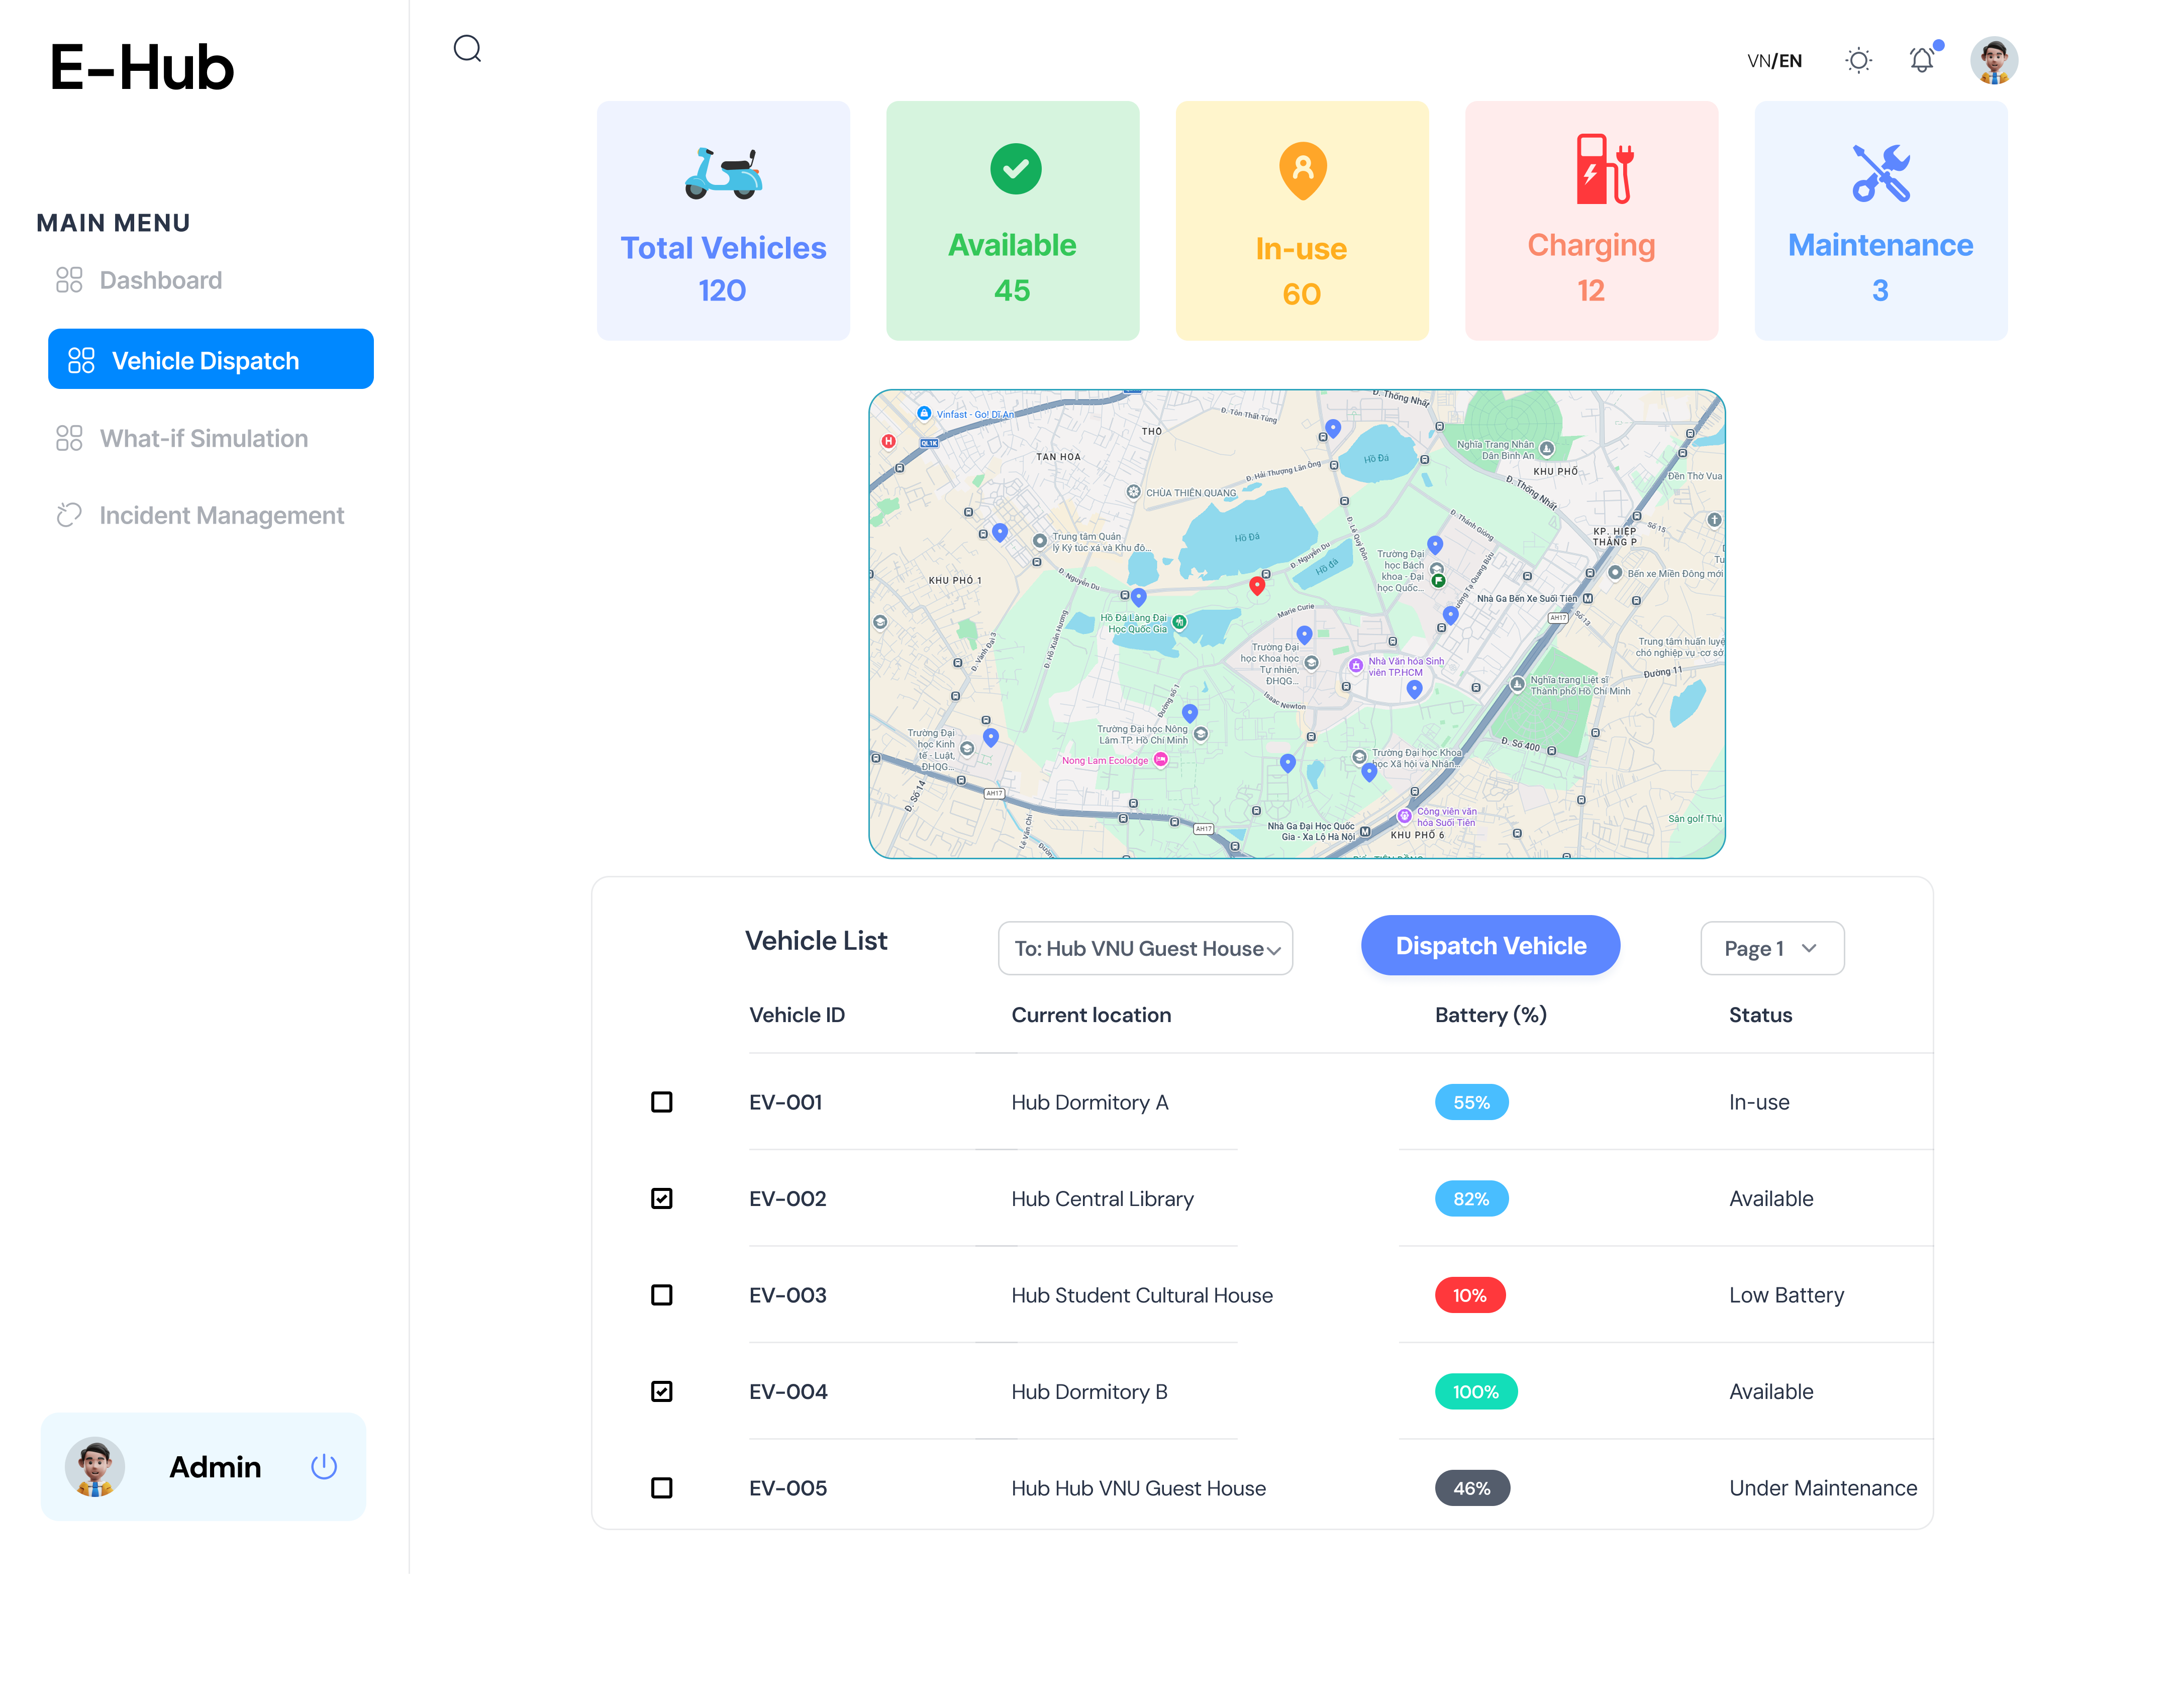
\includegraphics[width=0.96\linewidth,height=0.4\textheight,keepaspectratio]{s2/UI/DispatchScreen.png}
\captionof{figure}{Màn hình lập lệnh điều phối phương tiện giữa các Hub (UC11).}
\label{fig:dispatch_screen}
\par\vspace{0.5em}
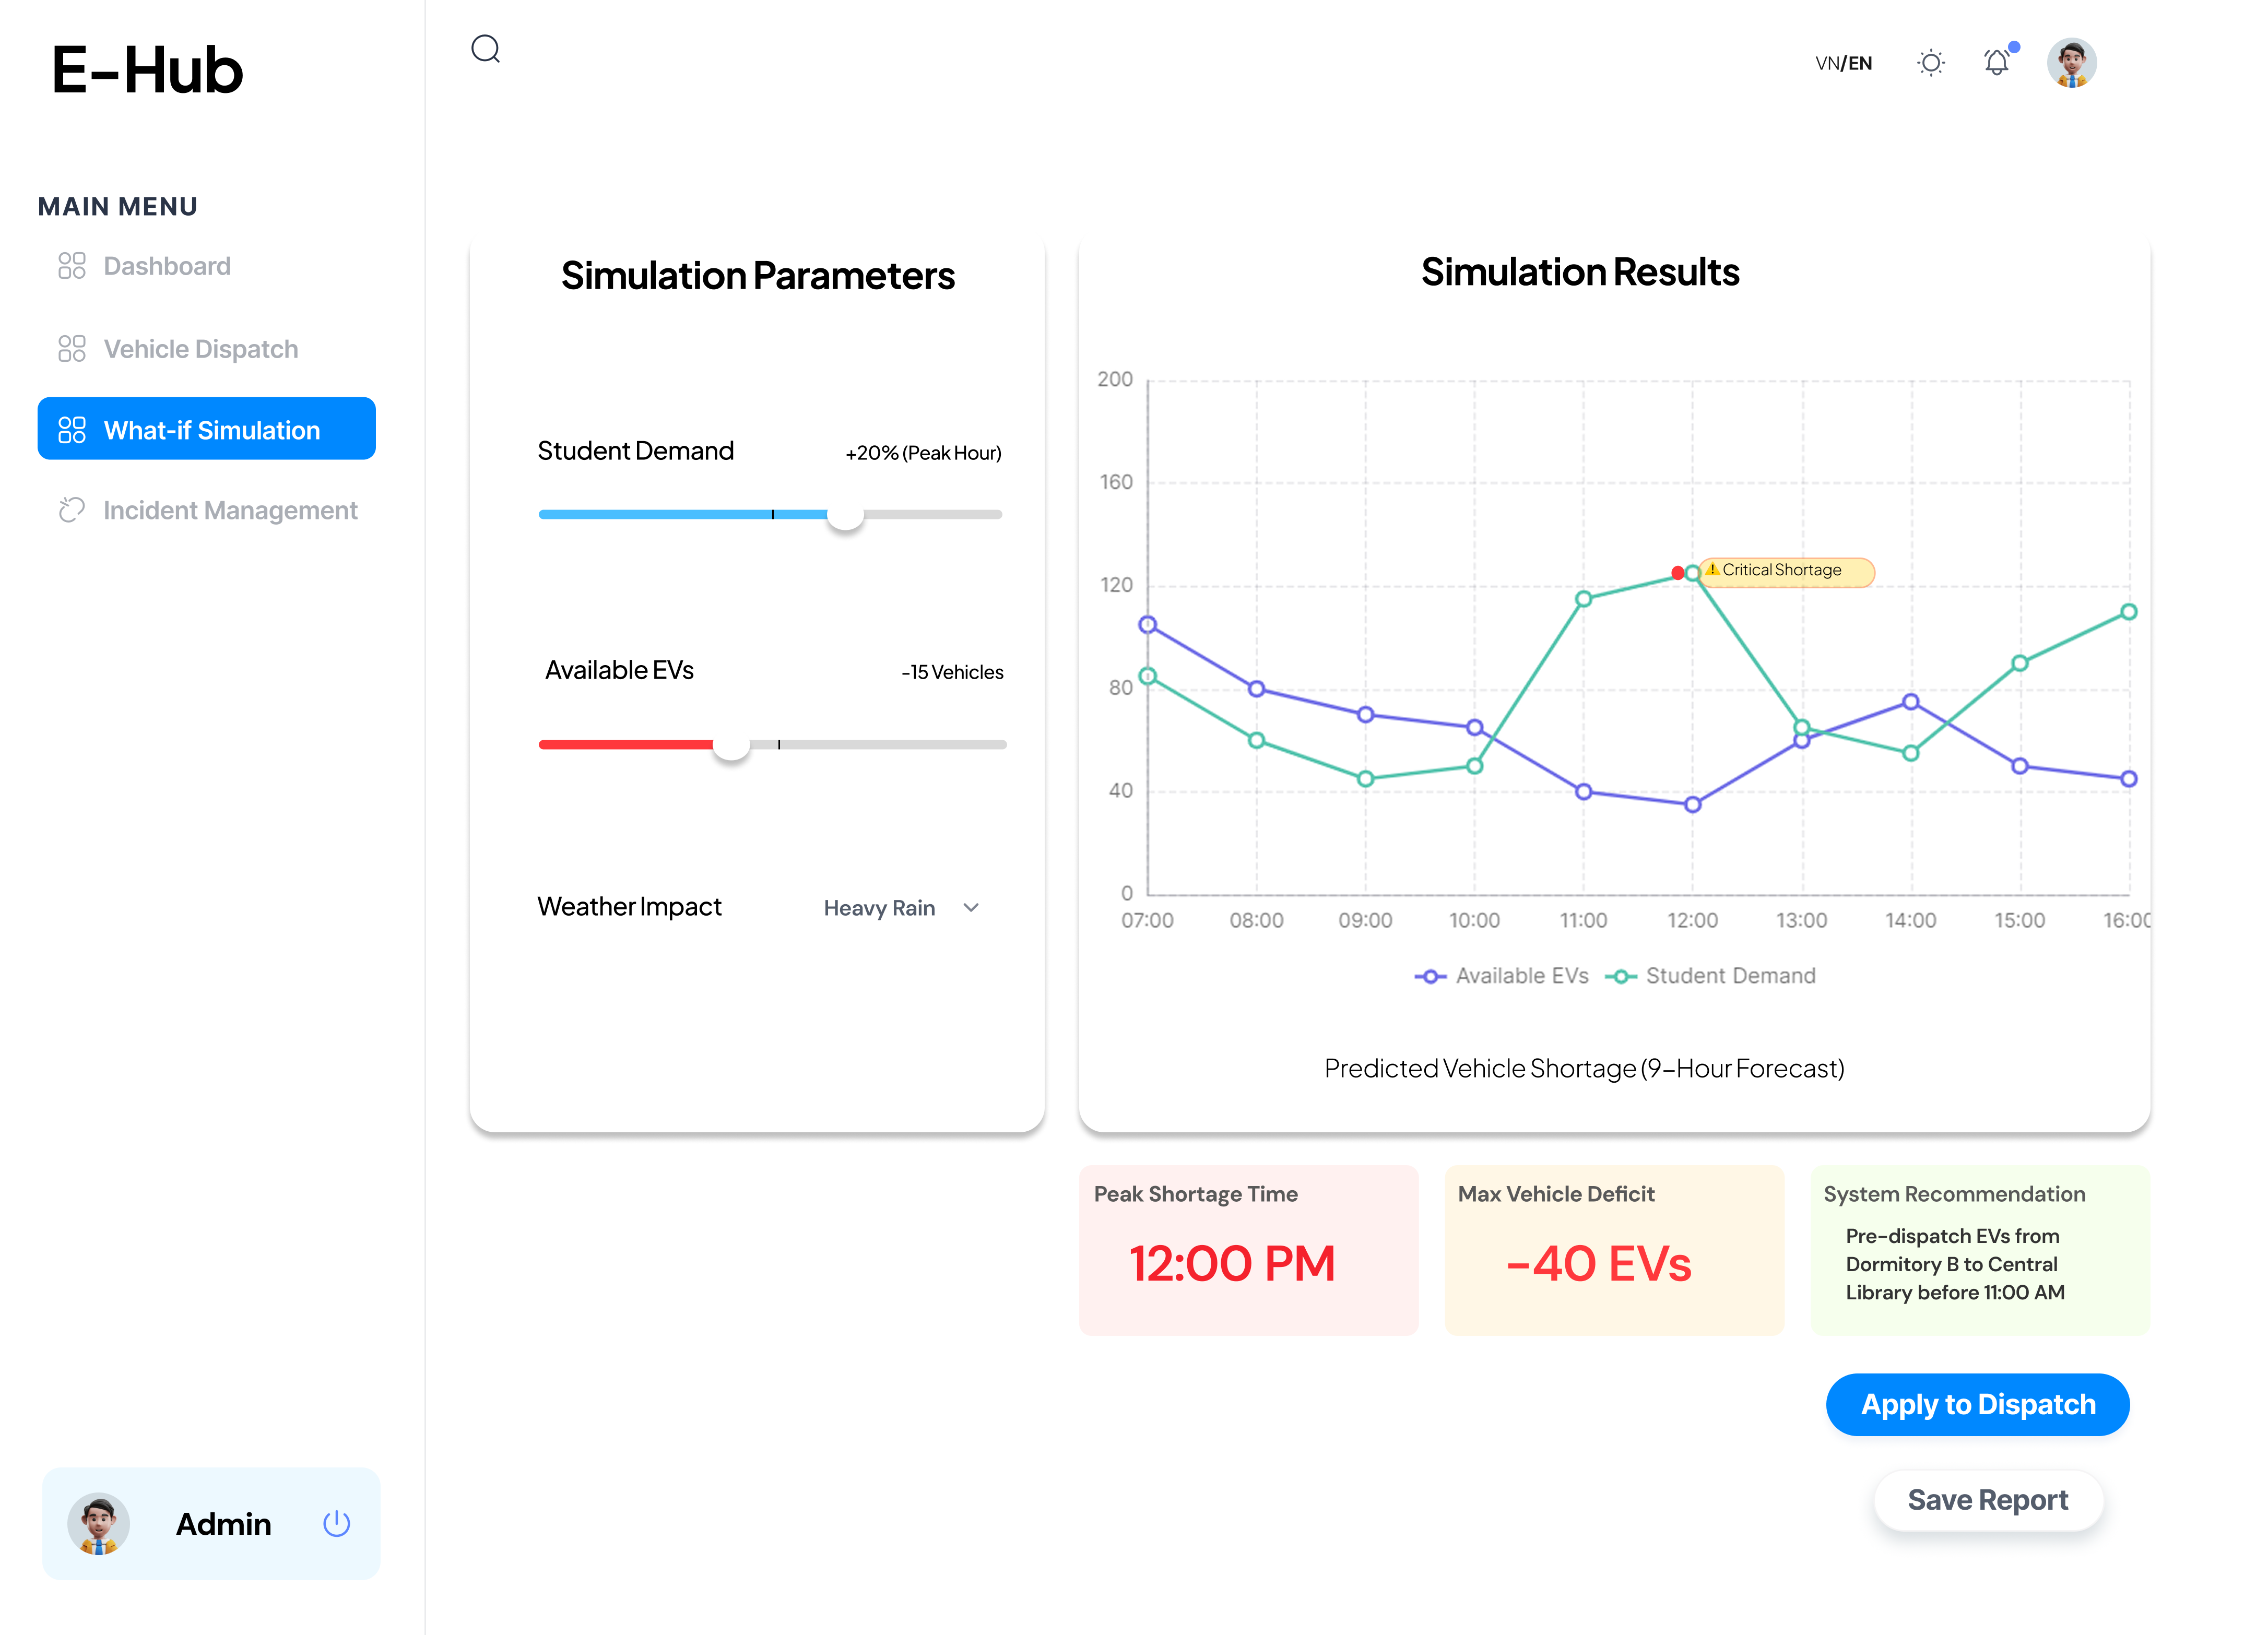
\includegraphics[width=0.96\linewidth,height=0.4\textheight,keepaspectratio]{s2/UI/SimulationPanel.png}
\captionof{figure}{Panel mô phỏng kịch bản What-if và dự báo nhu cầu (UC13, UC14).}
\label{fig:simulation_panel}
\end{figure}
\clearpage
\restoregeometry

\clearpage
\section{ACTIVITY DIAGRAM}

\insertsplitdiagram{ACTIVITY_DIAGRAM/AD1_1.drawio.png}{ACTIVITY_DIAGRAM/AD1_2.png}{Activity Diagram AD1 .}{fig:activity-ad1}
\insertdiagram{ACTIVITY_DIAGRAM/AD2.drawio.png}{Activity Diagram AD2.}{fig:activity-ad2}
\insertdiagram{ACTIVITY_DIAGRAM/AD3.drawio.png}{Activity Diagram AD3.}{fig:activity-ad3}
\insertdiagram{ACTIVITY_DIAGRAM/AD4.drawio.png}{Activity Diagram AD4.}{fig:activity-ad4}
\insertdiagram{ACTIVITY_DIAGRAM/AD5.png}{Activity Diagram AD5.}{fig:activity-ad5}
\insertdiagram{ACTIVITY_DIAGRAM/AD6.png}{Activity Diagram AD6.}{fig:activity-ad6}
\insertdiagram{ACTIVITY_DIAGRAM/AD7.png}{Activity Diagram AD7.}{fig:activity-ad7}
\insertdiagram{ACTIVITY_DIAGRAM/AD7E.png}{Activity Diagram AD7E -- UC7 AF3: Sạc khẩn cấp.}{fig:activity-ad7e}
\insertdiagram{ACTIVITY_DIAGRAM/AD8.png}{Activity Diagram AD8.}{fig:activity-ad8}
\insertdiagram{ACTIVITY_DIAGRAM/AD9.png}{Activity Diagram AD9.}{fig:activity-ad9}
\insertdiagram{ACTIVITY_DIAGRAM/AD10.png}{Activity Diagram AD10.}{fig:activity-ad10}
\insertdiagram{ACTIVITY_DIAGRAM/AD11.drawio.png}{Activity Diagram AD11.}{fig:activity-ad11}
\insertdiagram{ACTIVITY_DIAGRAM/AD12.png}{Activity Diagram AD12.}{fig:activity-ad12}
\insertdiagram{ACTIVITY_DIAGRAM/AD13.drawio.png}{Activity Diagram AD13.}{fig:activity-ad13}
\insertdiagram{ACTIVITY_DIAGRAM/AD14.drawio.png}{Activity Diagram AD14.}{fig:activity-ad14}
\insertdiagram{ACTIVITY_DIAGRAM/AD15.png}{Activity Diagram AD15.}{fig:activity-ad15}
\insertdiagram{ACTIVITY_DIAGRAM/AD16.png}{Activity Diagram AD16.}{fig:activity-ad16}
\insertdiagram{ACTIVITY_DIAGRAM/AD17.png}{Activity Diagram AD17.}{fig:activity-ad17}

\clearpage
\section{SEQUENCE DIAGRAM}

\insertsplitdiagram{SEQUENCE_DIAGRAM/SD1_1.png}{SEQUENCE_DIAGRAM/SD1_2.png}{Sequence Diagram SD1 .}{fig:sequence-sd1}
\insertdiagram{SEQUENCE_DIAGRAM/SD2.drawio.png}{Sequence Diagram SD2.}{fig:sequence-sd2}
\insertdiagram{SEQUENCE_DIAGRAM/SD3.drawio.png}{Sequence Diagram SD3.}{fig:sequence-sd3}
\insertdiagram{SEQUENCE_DIAGRAM/SD4.drawio.png}{Sequence Diagram SD4.}{fig:sequence-sd4}
\insertdiagram{SEQUENCE_DIAGRAM/SD5.png}{Sequence Diagram SD5.}{fig:sequence-sd5}
\insertsplitdiagram{SEQUENCE_DIAGRAM/SD06_Pic1.png}{SEQUENCE_DIAGRAM/SD06_Pic2.png}{Sequence Diagram SD6 .}{fig:sequence-sd6}
\insertsplitdiagram{SEQUENCE_DIAGRAM/SD07_Pic1.png}{SEQUENCE_DIAGRAM/SD07_Pic2.png}{Sequence Diagram SD7 .}{fig:sequence-sd7}
\insertdiagram{SEQUENCE_DIAGRAM/SD07E_SacKhanCap.png}{Sequence Diagram SD7E -- UC7 AF3: Sạc khẩn cấp.}{fig:sequence-sd7e}
\insertdiagram{SEQUENCE_DIAGRAM/SD8.drawio.png}{Sequence Diagram SD8.}{fig:sequence-sd8}
\insertdiagram{SEQUENCE_DIAGRAM/SD9.drawio.png}{Sequence Diagram SD9.}{fig:sequence-sd9}
\insertdiagram{SEQUENCE_DIAGRAM/SD10.drawio.png}{Sequence Diagram SD10.}{fig:sequence-sd10}
\insertdiagram{SEQUENCE_DIAGRAM/SD11.drawio.png}{Sequence Diagram SD11.}{fig:sequence-sd11}
\insertdiagram{SEQUENCE_DIAGRAM/SD12.drawio.png}{Sequence Diagram SD12.}{fig:sequence-sd12}
\insertdiagram{SEQUENCE_DIAGRAM/SD13.drawio.png}{Sequence Diagram SD13.}{fig:sequence-sd13}
\insertdiagram{SEQUENCE_DIAGRAM/SD14.drawio.png}{Sequence Diagram SD14.}{fig:sequence-sd14}
\insertdiagram{SEQUENCE_DIAGRAM/SD15.png}{Sequence Diagram SD15.}{fig:sequence-sd15}
\insertdiagram{SEQUENCE_DIAGRAM/SD16.png}{Sequence Diagram SD16.}{fig:sequence-sd16}
\insertsplitdiagram{SEQUENCE_DIAGRAM/SD17_Pic1.png}{SEQUENCE_DIAGRAM/SD17_Pic2.png}{Sequence Diagram SD17 .}{fig:sequence-sd17}

\clearpage
\section{STATE CHART}

\insertdiagram{cho_do_xe_state-chart.drawio.png}{State chart chỗ đỗ xe}{fig:state-chart-cho-do-xe}
\insertdiagram{cong_sac_state-chart.drawio.png}{State chart cổng sạc}{fig:state-chart-cong-sac}
\insertdiagram{xe_dien_state-chart.drawio.png}{State chart xe điện}{fig:state-chart-xe-dien}

\endgroup